% 26.07.18 Fallacies about physiology
\iflatexml
\else
\minitoc
\fi

\chapter{Fallacies\label{ch:Physiology-Fallacies}}

\quotationbox{
"And therefore when we go to investigate we shouldn’t pre-decide what it is we are trying to do except to find out more about it."
"The first principle is that you must not fool yourself, and you are the easiest person to fool."\\
-- Richard P. Feynman
}

As we mentioned, when discovering new facts and more details,
not only do they need to be inserted into the existing set,
but the validity of \textit{all} assumptions and approximations must be revisited.
Maybe the discovery supersedes one or more of the old items,
provides a new hypothesis in place of an old one,
turns a hypothesis into fact,
or question marks the overall validity (at least part) of the set of
approximations and abstractions. Alternatively, it turns a hypothesis into a \hypertarget{PhysiologyFallacy}{fallacy}.


Neuroanatomy provided an unbelievable wealth of details about the
\gls{CNS},
its structure, components, their infinite variety of implementation,
connection, chemical/enzymatical composition, and so on.
A vast amount of data is collected and available,
and uncountable attempts (mathematical models) have been made
to describe the actual phenomena. However, focusing on too many details
prevents understanding that \textit{"the nervous systems adopts
a number of basic principles"}~\cite{JohnstonWuNeurophysiology:1995}.
The illusion of having an imposing
knowledge base inspired undertakings such as simulating the entire human brain.
\index{brain!simulating}

The brain must be studied "from Inside Out"~\cite{BuzsakiTheBrain:2019}.
First of all, understanding how the known and established physical laws
underpin the operation of single neurons (the interface of non-living matter
and living matter) instead of hypothesizing additional laws and phenomena
complementing/overwriting them, led to creating a fictive nature, which in some points
resemblant to the real one. The abstraction, the discrete components connected
by ideal wires that can describe electric phenomena, is successful in electronics. However, it is not valid for neurons (see mainly the electrotonic models),
although some rough resemblance indeed exists.
The basic differences are that  \textit{the structure of living matter is different and
that many interactions with drastically different interaction speeds
are behind the phenomena}, as contrasted with the (mostly) single interaction
with a single speed of electronics.
\index{electrotonic model}
\index{living matter}

\textit{Nature is based on the collective operation of single neurons
and is prepared to consider the finite operating and transmitting times and uncertainties/failures of operation, unlike (most) technical networks}.
However, the usual neural network models~\cite{BrainNetworkModels:2018}
do not consider those differences.

%Last edited 2026.02.21
% Evaluating the Hodgkin-Huxley model

\section{Hodgkin\&Huxley's empirical description\label{sec:Physiology-HodgkinHuxley}}


We admire the contribution of Hodgkin and Huxley,
and especially that they were wery critical concerning the validity ot their own quantized observations. They admitted that their model was not correct in some aspects. However,
their followers made their works the 'Holy Bible' of physiology,
with their really bright ideas and some wrong choices they made. In this section we summarize their 'model', given that the fallacies discussed in this chapter are the direct consequences of some mistakes in the model.

As we discuss in section~\ref{sec:Physics-Electricity}, the body's electric signals
were discovered early, the principles, notions and technical equipments have been elaborated.
Even, some meticulous measurements correctly interpreted some of its signals. 
The development of electronical technology enabled their systematic study 
in the beginning of the 50's. However, experimenters 
often forgot that "\textit{Under ideal
circumstances, the physical act of measuring a neurophysiological event
would have no effect on the electrical signal of interest. Unfortunately,
this is seldom the case in neurophysiology.}"~\cite{JohnstonWuNeurophysiology:1995}.
	

The first systematic attempt to describe the results of observations in terms of the well-known laws of electricity
 was published around 1952~\cite{HodgkinHuxley:1952}.
A collection of their (modernized) papers is available~\cite{CompanionGuideHodgkinHuxley:2022}.
They made a huge amount of \hypertarget{HHmeasurements}{meticulous measurements}
and wanted to help the science community with providing equations for practical applicability.
To speed up reaching that goal, they introduced \textit{empirical functions} 
and derived equations, which, not surprisingly, described the \textit{empirical observations} quite accurately. 
The importance of their work is best highlighted by that it inspired 
different disciplines for discussion. 

\quotationbox{
"although highly successful
in predicting and explaining many of the electric characteristics of the action
potential, the HH model, nevertheless cannot accommodate the various non-
electrical physical manifestations (mechanical, thermal and optical changes)
that accompany action potential propagation, and for which there is ample
experimental evidence.~\cite{NerveSignalAsWindow:2023}
}

A technical reason is described in~\cite{HodgkinMemoryBook:1992}:
"The fact that the whole process for calculation of a $4-5\ ms$ interval,
showing the initiation of and recovery following an action potential, could be accomplished in 8 hours is astonishing."
The must-be oversimplification does not belong to the core of the theory.
When using the recent computing systems, not necessarily the old oversimplified models should be coded.
One could also use modern, more compute intensive, and physically correct models.

\subsubsection{Model summary\label{sec:Physiology-HodgkinHuxleyModelSummary}}
\begin{figure}
\centering
	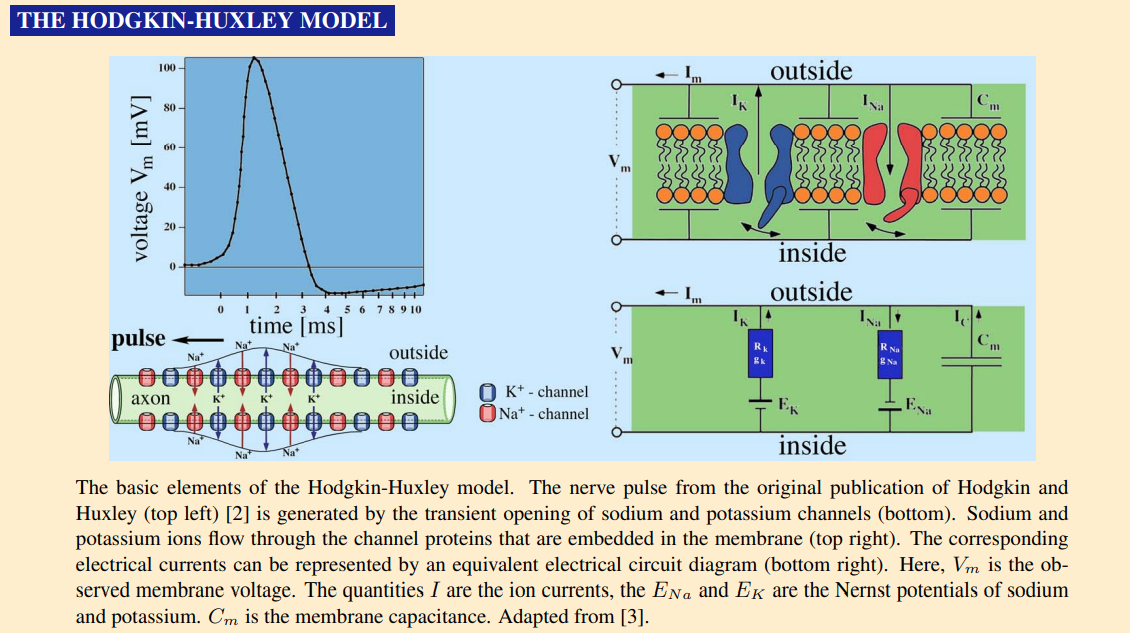
\includegraphics[width=\textwidth]
	{fig/HHModelHeimburg.png}
	\caption{The Hodgkin-Huxley model as reproduced by~\cite{HeimburgPhysikOfNerves:2009}}
	\label{fig:HHModelSummary}
\end{figure}


\subsubsection{Self-evaluation\label{sec:Physiology-HodgkinHuxleySelfEvaluation}}
In their brilliant publication~\cite{HodgkinHuxley:1952}, 
Hodgkin and Huxley evaluated their results "that our equations [must not be taken as] anything more than an empirical
description" and "the [partial] success of the
equations is no evidence in favour of the mechanism". 
When validating their observations,
they have found serious question marks: "a number of points were noted on which the calculated behaviour of our model
did not agree with the experimental results. We
shall now discuss the extent to which these discrepancies can be attributed to
known shortcomings in our equations."
"One was that the membrane capacity was assumed to
behave as a \textit{'perfect' condenser}, \dots the other was
that the equations governing the potassium conductance do not give as much
\textit{delay in the conductance rise} on depolarization as was observed in voltage clamps".
They did have the intuition that something was wrong and they correctly guessed its reason:
"it seems difficult to escape the conclusion that the changes
in ionic permeability depend on \textit{the movement of some component} of the
membrane \textit{which behaves as though it had a large charge}.\dots it is necessary to suppose
that \textit{there are more carriers and that they react or move more slowly} \dots \textit{there is no evidence from our
experiments of any current associated} with the change in sodium permeability, apart from the contribution of the sodium ion itself".

They emphasized that their work 
"must not be taken as evidence that their equations are anything more than an empirical description".
They made the first step of "a great journey into the unknown" and were very cautious by saying
that "the success of the equations is no evidence in
favour of the mechanism that they tentatively had in
mind when formulating them".

In his late work~\cite{HodgkinMemoryBook:1992}, Hodgkin evaluated the filtered experiences:
"We soon realized that \textit{the carrier model could not be made to fit certain results},
for example the nearly linear instantaneous current voltage relationship, and
that it had to be replaced by some kind of voltage-dependent gate. As soon as
we began to think about molecular mechanisms it became clear that
\textit{the electrical data would by themselves yield only very general information} about the class
of system likely to be involved. So we settled for the more pedestrian aim of
finding a simple set of mathematical equations which might plausibly represent
the movement of electrically charged gating particles."


\subsubsection{Nobel-laudation\label{sec:Physiology-HodgkinHuxleyNobel}}

Unfortunately, they also attempted to understand which physical processes happen in the membrane,
but they concluded with the feeling that "\textit{the interpretation given is unlikely to provide a correct picture of the membrane}."
Despite their explicite warning, that "the success of the equations is no evidence in
favour of the mechanism that we tentatively had in
mind when formulating them". 
Despite, they received the Nobel-prise "for their discoveries concerning the
\textbf{ionic mechanisms} involved in excitation and inhibition in the peripheral and central portions of the nerve".
As the philosphical approach to their work discusses, "One could dismiss this curious passage as scientific modesty
if it were not for the fact
that Hodgkin and Huxley argue for their conclusions."~\cite{MechanisticModelHodgkinHuxleyCraver:2006}
The science community rushed to apply the equations, instead of validating them.
To compensate for the disagreements with the experimental data, further ad-hoc
assumptions have been introduced, making their admittedly wrong picture even worse.

In the sense of philosophy, "there is a widely accepted distinction between
\textit{merely modeling a mechanism’s behavior} and \textit{explaining} it.
The equations
must be supplemented by a causal interpretation: one might, for example, agree by
convention that the effect variable is represented on the left, and the cause variables
are represented on the right, or one might add “these are not mere mathematical
relationships among variables but descriptions of causal relationships in which this
variable is a cause and this other is an effect,” and not vice versa",
for more details see~\cite{MechanisticModelHodgkinHuxleyCraver:2006,Mechanistic_HodgkinHuxley_2008}.
The lack of causality is one reasons why
HH have had the feeling they missed the correct picture of the membrane.
The other reason is that some fine details of their oversimplified picture was not accurate,
althought the additional (and arbitrary) ad-hoc assumptions have hidden the disagreements.
The followers have "fitted elephants"~\cite{FittingElephants:2021} by adding many more ad-hoc effects with too many parameters.

\subsection{Measurement science\label{sec:Physiology-HHPhilosophy}}

As highlighted in ~\cite{MechanisticModelHodgkinHuxleyCraver:2006}, the performed a very meticulous analysis
and characterized the time-course of the action potential phe
nomenally terms of different features (the concise listing taken from~\cite{MechanisticModelHodgkinHuxleyCraver:2006})

\begin{itemize}
\item the form, amplitude, and threshold of an action potential;
\item the form, amplitude, and velocity of a propagated action potential;
\item the form and amplitude of the resistance changes during an action potential;
\item the total movement of ions during an action potential;
\item the threshold and response during the refractory period;
\item the existence and form of subthreshold responses;
\item the production of action potentials after sustained current injection (that is,
anodal break);
\item the subthreshold oscillations seen in the axons of cephalopods
\end{itemize}


"A measurement can be precise without being accurate."\cite{JohnstonWuNeurophysiology:1995} \textit{Accuracy means characterizing 
the true measurable quantity.} In this sense, their measurement is precise but not accurate: they measured precisely wrong quantities, which, unfortunately, can be made and thought sufficiently resemblant to the real ones. 

\subsection{Mathematics\label{Physiology-HHMathematics}}
"These equations and the methods that arose from this combination of modeling and
experiments have since formed the basis for every subsequent model for active cells.
The Hodgkin-Huxley model and a host of simplified equations  derived from
them have inspired the development of \textit{new and beautiful mathematics}." \cite{MathNeuroscience:2010}.


\subsection{Physics\label{Physiology-HHPhysics}}

"A. L. Hodgkin and A. F. Huxley published what was to become known as the
model of the action potential. This model would subsequently be considered a cornerstone of
electrophysiology and neuroscience, since it concerned the ionic mechanisms involved in the
operation of the nerve cell membrane."~\cite{PhysicsForHodgkinHuxley:2024}




\subsubsection{Neglecting Coulomb's Law\label{Physiology-HHNeglectingCoulomb}}

\index{Coulomb's law}

\subsection{Driving force\label{sec:Physiology-HHDrivingForce}}



As we discuss in section~\ref{Physics-OscillatorIntegrator}, HH introduced 
by their Eq.~(1) (reproduced by us as Eq.~(\ref{eq:OutputHH}))
the basic decription of \textit{the membrane current \textbf{during a voltage clamp}} with that 
"the justification for this equation is that it is the simplest which can be used
and that it gives values for the membrane capacity which are independent of
the magnitude or sign of $V$ and are \textit{little affected by the time course of $V$}".
(It is again a reversed approach: the capacity, per definitionem, means the ability to store charge
and is one of the attributes of the medium instead of the electric characteristic
of the tested circuit. For the case of \hyperlink{voltage-clamping}{clamping}, it is an approximation
that the temporal course of the clamping voltage
is kept constant, the current remains constant.  
As we discuss in section~\ref{sec:Physiology-NeuralCurrentsPATCHING},
in the case of a constant current where $I=\frac{dQ}{dt}$,  the voltage increase $dV$
on the capacity $C$ of the membrane is $\frac{dQ}{C}=\frac{I*dt}{C}$,
so we can derive the "driving force" (compare it to Eq.~(\ref{eq:Nernst-dVdt}))
as they interpreted it
%
\[\frac{d}{dt} V=\frac{I}{C}\label{eq:Physiology-HHDrivingForce}\]
%
The direct \textit{constant} current input $\frac{d}{dt} V_{PATCH}$
to the neuron cell body is a simple constant current that causes a constant membrane's voltage derivative contribution.
That is, if one checks the dependence of the output voltage on $\frac{d}{dt} V$ and $I$, in the presence of a constant $C$,
one observes the same dependence.
However, the currents are not necessarily constant.





\section[The outward $K^+$ component during the \gls{AP}]
{The outward $K^+$ component during the \gls{AP}\label{sec:Physiology-Fallacies-OutwardK}}

One of the big mysteries in the creation of the V1.0  model was why \gls{AP}
became negative when only
$Na^+$ influx was seen when \gls{AP} was formed. 
Given that \gls{HH} found only positive charges nearby, they supposed that
an outflux of positive charges, namely of $K^+$ ions,  was the reason.
Since the process was too fast, \gls{HH} used a voltage clamping method (see section~\ref{sec:PHYSICS_clamping}) for the experimental demonstration~\cite{HodgkinHuxleyCurrent:1952} of the hypothesized  $K^+$ current. The essence of this is that they
imitated the crossing of the membrane voltage threshold (reaching the "AP" state, see Fig.~\ref{fig:ClampingKCurrent}):
"(after completion of the quick pulse through the membrane
capacity)", then raised the intracellular domain of the membrane to a potential higher than the resting potential with a negative feedback circuit:
"the potential
difference across the membrane is suddenly changed from its resting
value, and held at the new level by a feed-back circuit ('voltage clamp' procedure)", and measured the time dependence of the current in this state.

\subsection[The formal description of the process]
{The formal description of the process\label{sec:Fallacies-OutwardKPhysicsFormal}}

Figure \ref{fig:RestingPotential5} shows the changes that occur in a neuron that is displaced from its equilibrium state.
These processes are naturally slow, their role in the
transient process is discussed in the \hyperlink{TransientState}{transient state section},
here we only illustrate our statements regarding the $K^+$ current.
Our statement is essentially based on Kirchhoff's Voltage Law,
according to which the sum of the voltages in a closed circuit is zero.
 In our case, the circuit extends from the inside of the neuron to the external environment.
If for any reason the external and internal potential levels are not the same, then a current flows until they are equalized (current carries charge and causes a potential change; it is not an ideal voltage generator).
Of course, the equalization is not
instantaneous, the current has a time dependence.

On both the left and right sides of the figure, the resting potential level is
at the zero value of the vertical scale. In the resting state (without invasion),
in the intracellular segment
the [Na50,K400] concentrations are present inside the cell. Using these values, we reach the "Rest"
state along the green arrows (based on the Nernst voltages, see \ref{Tab:SummaryTable}~Table), which is located at a height of \SI{-21}{\milli\volt}.
On the right side, in the extracellular segment, from the point also at a height of 0, we arrive at a point at a height of \SI{21}{\milli\volt} along the blue arrows in the same way. The potential difference between the two mentioned points is \SI{42.5}{\milli\volt}, which \gls{HH} measured. It is a correct value,
but it is the result of an electrostatic charging and not of a voltage drop due to the "leakage current" they assumed.
\index{leakage current}
The voltage across the membrane (represented by the solid orange arrow) points upwards, preventing positive ions in the intracellular space from moving towards the extracellular space and preventing negative ions in the extracellular space from moving towards the intracellular space. The $Ca^{2+}$ ions in the extracellular segment, however, are permeable, requiring continuous pumping. There is no potential difference between the outside and inside, so no (significant) current flows.

If, for any reason, the membrane voltage suddenly rises above the threshold value, due to the extremely fast $Na^+$ influx,
the membrane potential increases by about \SI{100}{\milli\volt} (a [Na200,K400] state occurs, see the brown arrows), i.e. the neuron jumps into the AP bubble.
%After the threshold is exceeded naturally or with a short pulse, the "AP" passes into the "Rest" bubble,
%this is the same in the case of natural and clamping measurements.
The orange arrow that was pointing upwards now points downwards as a broken line: the outflow of positive ions (both $K^+$ and $Na^+$) is given a free path, but the sloping path for $Ca^{2+}$ ions is eliminated. However, the free ions in the surface layer of the membrane are the vast majority of the $Na^+$ ions that have just arrived, so the ion current through the \gls{AIS} mainly consists of such ions.
A significant increase in the membrane voltage leads to a significant increase in the potential of the
inner space of the neuron.
A current is initiated that tries to restore the initial voltage and concentration relationships.
The extracellular environment of the membrane is extremely stable (the concentrations do not change),
but inside the cell the voltage increases to the same extent, in the direction of "Invasion".
The membrane potential has changed significantly due to the change in the $Na^+$ concentration, so the cell then moves them towards equilibrium.

\begin{figure}
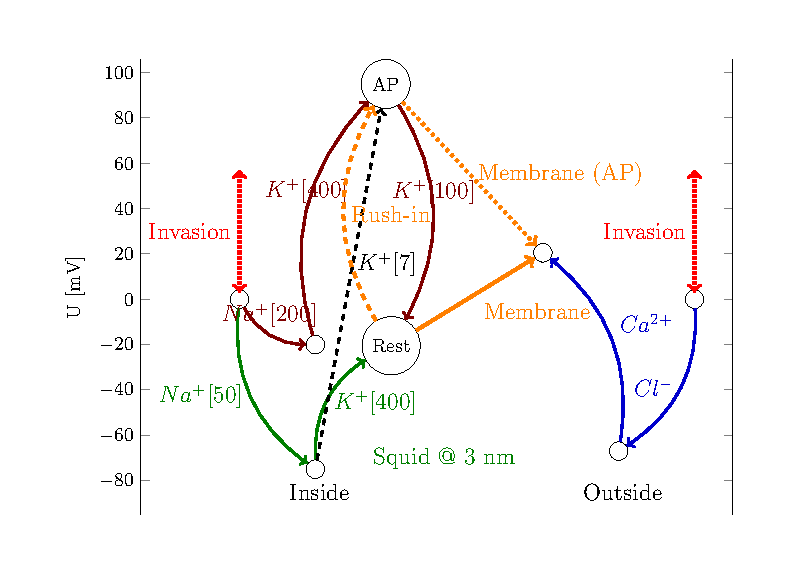
\includegraphics[width=.9\columnwidth]{fig/RestingPotential5.pdf}
\caption{The figure is a modified version of Fig.~\ref{fig:RestingPotential4}. It is supplemented with the unbended black line showing that the clamping condition forces the neuron
to find a new balanced state by compensating the clamping voltage
with setting a concentration [Na50,K7].
For comparison, the case of natural \gls{AP} is also shown.
The mechanism of producing \gls{AP} (using numbers referring to the case of squid shown in Table~\ref{Tab:SummaryTable}). In the resting state, the inside thermal potentials follow the green paths.
When the rush-in of $Na^+$ ions suddenly increases the internal concentration to $[200]$, the potential on the internal side of the membrane increases to $+90\ mV$. The neuron must decrease its concentrations to restore the resting potential, mainly by releasing an action potential through the \gls{AIS}.
The clamping fixes neuron's membrane voltage at \gls{AP},
so the neuron can operate only with the concentrations.
\label{fig:RestingPotential5}
}
\end{figure}

In the case of natural \gls{AP}, there is no obstacle for the neuron
to restore its previous state by changing any parameter, so the system concentrations
start towards the state [Na50,K400]. This can be
easily achieved by trying to make Na[50] from Na[200], while $K^+$ is still/already at the appropriate concentration.
That is, it releases (mainly) $Na^+$ ions through the \gls{AIS} until the potential difference drops to zero.
Reducing the $Na^+$ concentration also reduces the membrane
voltage, i.e. after the release of the excess ions (admitted during the $Na^+$ rush-in) the neuron returns to its initial state;
a cycle takes place.

"Clamping" fixes the membrane voltage, meaning that the neuron cannot restore its initial
resting state. Instead, it has to find a new balance by changing the concentrations.
After the artificial \gls{AP}, clamping (using a negative feedback) keeps the membrane potential at a fixed value, so the neuron can only produce a new balance by changing the ion concentrations: a current flows until the Nernst voltages of the $Na^+$ and $K^+$ concentrations can balance the clamping voltage.
From this [Na50,K400] state, the neuron has to adjust the potential so that the sum of the Nernst voltages plus the membrane's voltage plus the clamping voltage is zero (so another balance has to be set!), while the voltage is fixed.
To do this, it must reduce the $K^+$ concentration, while the $Na^+$ concentration is already at a good value (the opposite of the previous case). And not by a small amount: [K7] only causes a voltage change equal to the clamping 100 mV imposed on the cell.
This voltage is given by the green curved $Na^+[50]$ and the black dashed straight
$K^+[7]$ path. The neuron can achieve this [Na50,K7] concentration
by starting an intensive $K^+$ release.

\begin{figure}
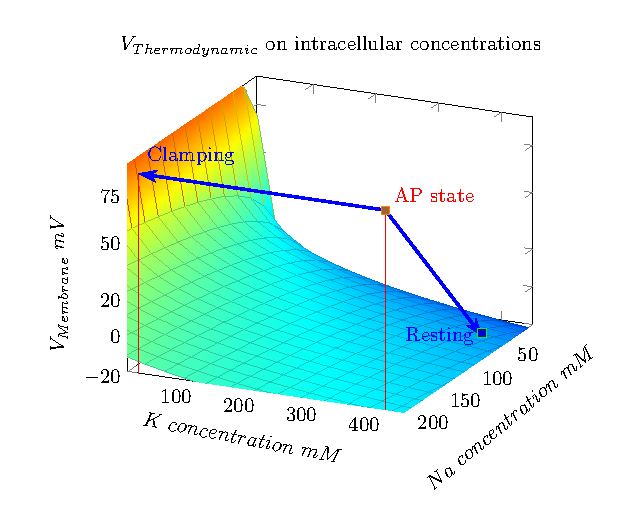
\includegraphics[width=.9\columnwidth]{fig/ClampingKCurrent.pdf}
\caption{Artificial and natural degradation of the AP state.
In the case of natural degradation, the neuron
has to get rid of the (unnecessary) $Na^+$ ions;
by releasing them, it returns to the initial state;
cycle takes place.
Clamping keeps the membrane voltage fixed,
so the neuron can only establish a new equilibrium situation by changing the intracellular concentrations
which, due to the very reduced $K^+$ concentration, is only possible with an intense
$K^+$ release.
\label{fig:ClampingKCurrent}
}
\end{figure}

Another important difference compared to the natural case is that there is no electrostatic acceleration across the membrane (which is why the $Na^+$ influx stopped),
only a thermodynamic suction effect outwards due to clamping.
Indeed, $K^+$ ions attempt flow out through the membrane, but
they cannot exit until the electric potential drops
below the equivalent thermodynamic driving force of the concentration.
Moreover, the nearby $K^+$ ions get there sooner, but they leave a gap (reduced concentration) behind them, where the nearby neighbor $K^+$ electrodiffuses. This is why the physiologist sees a "delayed current".
It is a strange game of nature that the resultant of the thermodynamic and the electric  (plus the elastic)  gradients moves, simultaneously, the $Na+$ ions parallel to the membrane surface, toward the \gls{AIS}, and
the $K^+$ ions perpendicular to the surface toward the membrane,
approximately until the peak of the action potential voltage is reached.
The $Na^+$ starts to leave through the \gls{AIS}, while the "excessive" $K^+$ ions leave through the membrane.
\textit{The two currents do not flow in the same path, so they cannot
interfere as currents in opposite directions and cannot cause hyperpolarization.}
\index{hyperpolarization}
Hyperpolarization is caused by the reversal of the $Na^+$ current, which can be interpreted
in the electrical sense as the capacitive current of the capacitor in the serial $RC$ circuit, and
in the mechanical sense as the negative period of the elastic membrane oscillation.

\textit{That is, the $K^+$ current is an artifact caused by the clamping, which is caused by the 'clamping' measurement conditions, and does not occur in the neuron under natural conditions.}


So, this is where the urban legend "$K^+$ flows out through the membrane in the second phase of \gls{AP}, with a significant delay compared to the $Na^+$ influx" comes from.
It is really a real measurement, it is really $K^+$ ion, but they did not measure what they thought.
\gls{HH} and their late descendants did too. So there is no question of specific $Na^+$ and $K^+$ (synchronized with each other) channels: in both cases, the concentration and potential relationships decide what ions flow and in which direction.
%It doesn't hurt to use a good model for what you want to study.
\gls{HH} was aware that theirs was not good, but they didn't know any better.
Unfortunately, they spread the misconception.



In the classic experiment of \gls{HH}, clamping means that the left-hand "Invasion" suddenly raises the membrane voltage to the peak value measured at \gls{AP}, without the concentrations changing, so the voltage of the left-hand segment will also be higher.
The current only stops when the difference in the Nernst voltages of the inner segments equalizes
the clamping voltage. Due to the slowness of charge carriers, the process is not instantaneous.

Fig.~\ref{fig:ClampingKCurrent} shows a pictorial summary of the process. The points on the surface give the Nernst voltage acting on the ions, for different combinations. The points on the surface are in equilibrium. The onset of the \gls{AP} moves the point that was in equilibrium until then well outside the surface. The neuron can find the new equilibrium position without the forcing effect of clamping by restoring the parameters of the previous state. In the case of clamping, it must set new concentrations at which the sum of the Nernst voltages can counteract the clamping voltage. In both cases, a relaxation process takes place, which in the case of the native process is measured by physiology as \gls{AP}.

% Compiled 26.07.10
\subsection[The physics of the process]
{The physics of the process\label{sec:Fallacies-OutwardKPhysics}}

The essential functioning of the cell largely takes place in layers of a few nanometers close to the cell membrane, where differences in concentration and voltage gradients (and consequently material flow rates) of up to several orders of magnitude can occur for a few dozen microseconds. Furthermore, the slow material flow creates potential and concentration changes that change from moment to moment, and whose effects can be significantly different in each layer due to the chemical quality of the ions. For this reason, the description of the events is unique in each case, for each layer and for each time period; it is not uncommon for scientific disciplines to be changed when describing individual stages, or for them to be combined in a different way.

The two ends of the ion channels embedded in the membrane have different potentials and concentrations, so that the ions passing through acquire significant energy and speed. However, this gradient disappears when they exit the channel, so that the ions "stop" in frustration. The passage continues until the passing ions increase the electrochemical potential of the other side so much that the gradient disappears. Inside the electrolyte, the other, orders of magnitude smaller gradients continue to operate, of course, but can only create very slow material transport. The changes in the "bulk" part of the electrolyte tend towards slow equalization (different rules remain in effect near the boundary membrane). For this reason, a slow diffusion effect is also associated with all processes.

When $Na^+$ ions penetrate the intracellular segment, they do so under the influence of a significant electrochemical gradient. In this way, immediately after the passage (lasting a few nanoseconds), the ions create a $Na^+$-rich layer, from which the charge of the ions (partly by direct collision) knocks out the ions there, mainly $K^+$.
Basically, a $Na^+$ layer is formed directly under the intracellular part of the membrane, which increases the voltage on the capacitor plates, and since the \gls{AIS} at the end of the membrane acts as a sink for the ion current, an immediate $Na^+$ current is initiated, as discussed in the electrical model.
$Na^+$ ions move along the membrane surface due to the high electrical gradient through the high-conductivity \gls{AIS}, but small amounts of $Na^+$ and $K^+$ ions apparently diffuse into the adjacent layer. The ion concentration and potential of the layer decrease with the outflow current. Due to the slowness of the ion current, the ions only reach the \gls{AIS} in tens of microseconds.
The membrane is initially closed to positive ions (after the $Na^+$ ions have passed through), and the $Na^+$ layer represents an additional potential barrier. However, over time, the decreasing $Na^+$ concentration due to the current in the layer that causes the \gls{AP} increasingly allows $K^+$ ions to move towards the membrane and the experienced $K^+$ current to start, which is only possible after a few dozen microseconds.

"Delayed $K^+$ channels" therefore mean ion channels that structurally do not distinguish between ions, and the delay is caused by transient processes taking place in the ion layers. These channels indeed release $K^+$ ions, which only start when the clamping voltage is switched on to the neuron (i.e., they create a non-equilibrium state of the neuron segment), and only $K^+$ ions because the thermodynamic gradient is only favorable to them.

\gls{HH} found that the \gls{AP} can be decomposed into two currents:
"the ionic current during a depolarization consists of two more or less independent components in parallel, an early transient phase of current carried by sodium ions, and a delayed long-lasting phase of current carried by potassium ions".
Their conclusion is more than surprising, that although the current component arising from Na ions appears quickly, the component consisting of $K^+$ ions remains delayed and persistent. According to that "explanation", the neurons are disposable devices: after emitting a single \gls{AP}, the neuron emits a short-lasting $Na^+$ and (according to their figures 5 and 6) an infinitely long-lasting $K^+$ current, contrary to experience.
In other words, for \SI{100}{\pico\ampere} (that is \SI{1e-10}{\ampere}) saturation current and \SI{1e11}{neuron} it would mean
10~amper permanent current in the brain.
Furthermore, it would keep the resting potential above 
the value of the resting potential. The difference 
would be the extra voltage of the clamping; that is,
it would disappear at zero claping voltage.
In other words, the extra voltage and the  $K^+$ current disappears in the absence of clamping, as observed.

In our reading the current lasts as long as the voltage invasion caused by clamping persists or the $K^+$ content of the intracellular segment of the neuron is depleted.


\section{Equivalent electrical circuit\label{sec:Fallacies-ElectricalCuircuit}}

"These ionic concentration gradients across the cell membrane
constitute the driving forces (or chemical potentials)
for ionic currents flowing through open channels in the membrane.
In other words, the ionic concentration gradients act like DC batteries
for cross-membrane currents.”~\cite{JohnstonWuNeurophysiology:1995}

%\subsubsection{Equivalent circuits\label{Physiology-HHEquivalentCircuits}}
%


\begin{figure}
\centering
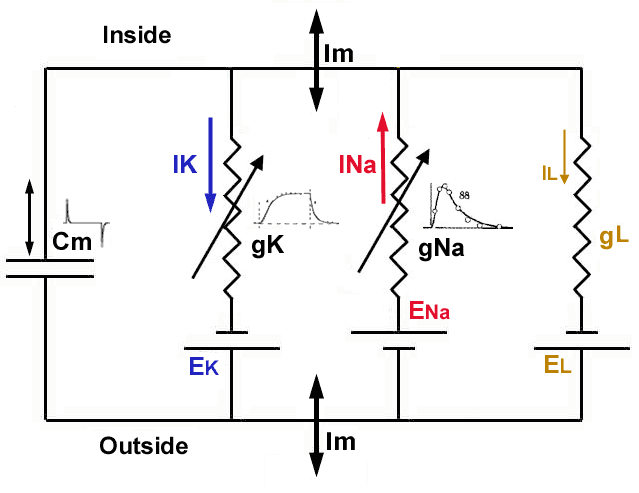
\includegraphics[width=.65\textwidth]{fig/HHcirdiagm.png} 
\caption{The equivalent circuit for the Hodgkin-Huxley model}
\label{fig:HH_EquivalentCircuit}
\end{figure}



%\subsection{Circuits\label{sec:Circuits}}
The biological 'equivalent circuit' models assume that the circuits comprise point-like
ideal \textit{discrete elements}
such as condensers and resistors, and some hidden power changes their parameters according to some
mathematical formulas,
furthermore ideal batteries with voltage that may again be changed  by that power.
All they are connected by conducting  (metallic) ideal wires
and their interaction speed is infinitely high (the Newtonian 'instant interaction').
Using that abstract model enables them to use the well-known classic equations, named after
Ohm, Kirchoff, Coulomb, Maxwell and others. However, those abstractions have severe limitations.
Biology applies Ohm's Law to its objects while claims that its objects are non-ohmic;
understands that neural currents comprise ions while claims that the ions do not feel the Coulomb repulsion;
measures ions' propagation speed but in its equations it claims that their effects are instant;
hypotesizes non-existing physical mechanisms to make their nature. In general,
biophysics abstracts from the world of the physics-inspired mathematical formulas a fictitious nature
where biology lives and hypothesises complementary mechanisms to achieve some resemblance with the true biological word.
The examples include that ions in the ions channels do not repulse each other;
that charge, potential and current are independent of each other;
that ion currents do not repulse each other neither when they travel from the presynaptic terminal to the
\index{Coulomb's law}
\gls{AIS};
that some hidden power opens the ion channels to let ions in into the intracellular space,
that ions with the same charge move in opposite directions when ions rush-in into the intracellular segment of the neuron;
that the ions pass ion channels without being accelerated by the potential difference accross the membrane;
the telegraph equations are applied to the case of axons although neither external potential nor current loss exists; and so on.


Even that unfortunate idea of equivalent circuits leads to analyzing
"electrotonic (electronic circuit equivalent) modeling of realistic neurons and the interaction of dendritic morphology
and voltage-dependent membrane properties on the processing of neuronal synaptic input"~\cite{SingleNeuronComputation:2014};
that is, to study a simulated neuron built from discrete electronic components. However, the idea needs to put together
many compone "raises the possibility that the neuron is itself a network". On the one side, such an idea misguides the neurophysical research (since actually a fake neural system is scrutinized, the validity of the approach is questionalized~\cite{RealisticNeuronalModeling:2016}), and on the other, since electroengineers understand
the neuronal operation from the wrong model, it also misguides building neuromorphic architectures. 

The equivalent circuits are a source of misinterpretations. As~\cite{JohnstonWuNeurophysiology:1995} formulates,
"In other words, the ionic concentration gradients act like DC batteries for cross-membrane currents."
We call the attention again, that \textit{ions} represent the current,
that is \textit{that current changes changes the concentration, that changes
the voltage of the DC battery, unlike in the case of the equivalent circuits}.
This difference is significant in understand how the basic neuronal circuit works.
Introducing equivalent circuits prevents explaining the fundamental 
electric phenomena.

%\quotationbox{
%This was how — Richard P. Feynman approached all knowledge: What can I know for sure, and how can I come to know it?
%It resulted in his famous quote, “\textit{You must not fool yourself, and you are the easiest person to fool.}”
%Feynman believed it and practiced it in all of his intellectual work.
%}
%\index{Feynman, Richard P.}


\section{Point-like neuron\label{sec:Physiology-FallaciesPointLike}}

The abstraction we need to use always includes simplifications and omissions,
depending on which phenomena we want to study. If we want to describe Earth's orbit around our Sun, we can consider it point-like at an elementary level and assume pairwise interaction between them.  However, for finer details, we need to consider its structure, size, and the disturbing effects of other planets and its Moon. Whether the abstraction of having point-like neurons is valid depends on the targeted phenomenon.

In the initial investigations, the \textit{size of the cells} was seen
to be much smaller than the \textit{size of their connections}.
In addition, the axons were much earlier available for experimental
investigations, suggesting that the observed signals originate and
terminate in the network nodes. This abstraction might be
appropriate (with some limitations, mainly due to the connection speed)
until we can develop technical tools to study the \textit{internal operation}
of the network nodes. "We assume that the dimensions
of the cell are small enough so that spatial variations in the membrane potential can be neglected"~\cite{KochBiophysics:1999}. Its internal operations and phenomena can only have an artificial timing, its input signals are artificially correlated, and its mystic internal operation produces an action potential as an output signal in a pair-wise interaction.

When starting from 'the so-called point representation
of a neuron" \cite{KochBiophysics:1999}, admitting that "such
an approximation would be valid, for instance, if we were investigating
a small, spherical cell without a significant dendritic tree", we
necessarily conclude that "individual neurons convert
the incoming streams of binary pulses into analog, spatially distributed
variables". This statement attempts to underpin that in the neural networks
digital pulses are traveling, which is less then the half of truth.
This point of view blocks the interpretation of even the phenomena that are correctly seen and leads to the design of wrong experiments. Among others, it results in the immediate consequence of interpreting neuronal communication as streams of binary pulses,
which leads to applying Shannon’s mathematical theory to neural communication, despite Shannon's sharp opposition~\cite{ShannonBandwagon:1956}.
\index{neuron!point-like}
\index{point-like neuron}
\index{Shannon, Claude}
\index{information theory!neural}
\index{neural information theory}




\section{Passive distributed membrane\label{sec:Physiology-FallaciesPassiveMembrane}}

The role of the neuronal membrane is controversial as used in physiology.
As \cite{KochBiophysics:1999}
discussed, 'from an electrical point of view, the properties of the membrane can be
satisfactorily described by a sole element: a capacitance.' However, on the same page, the
caption of Figure 1.1 explains that 'Proteins inserted into the membrane, here ionic channels,
provide a conduit through the membrane.' Also, the 'associated lumped electrical circuit for this patch,
consisting of a capacitance and a resistance \textit{in series} with a battery' (and parallel
with each other).
That picture is wrong; see Figure \ref{StructureOfAIS}.
When inventing the 
AIS, the wrong hypothesis turned into a fallacy.
\index{passive membrane}
\index{membrane!passive}


\begin{figure}
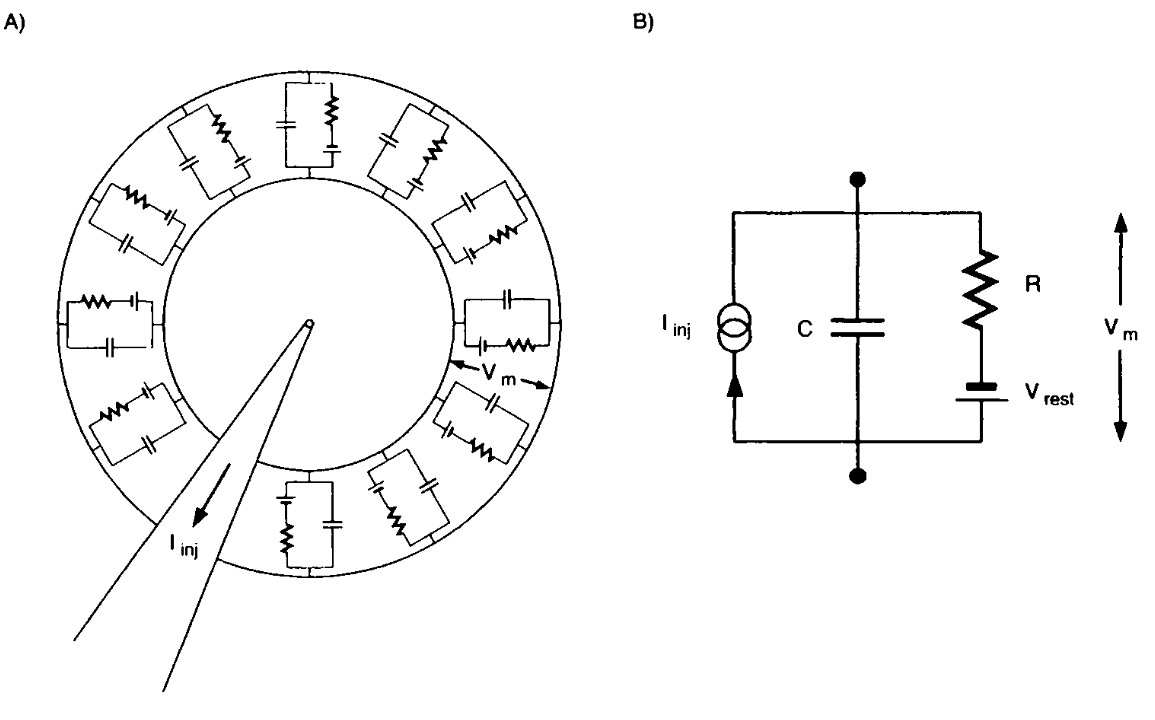
\includegraphics[width=.65\textwidth]{fig/PassiveNeuronMembraneCircular.jpg}

\caption{Equivalent electrical
model of a spherical cell with passive membrane. \cite{KochBiophysics:1999} Fig. 1.2 \label{fig:Fallacies-NeuronMembraneCircular} }
\end{figure}



\section{Membrane as a wrong isolator\label{sec:Physiology-Wrong isolator}}

When assuming that the membrane's resistance and capacitance are distributed over its surface,
one must also assume that it has imperfect resistance despite 
no known mechanisms to conduct an ionic current. The membrane is a perfect isolator
connected to a resistance the neuron's 
%\gls{AIS}
AIS
 represents. The ionic current
(although it is not a 'leaking current') can flow out through it. The right picture
that the capacitor and resistor are connected serially instead of parallel, as
introduced several decades ago, defies the fallacy that the membrane is a non-perfect isolator.

\section{Energy consumption\label{subsec:EnergyConsumption}}

The passive distributed membrane implies that in its resting state (without operation and communication), a permanent 'leaking current' flows out from the $RC$ circuit through the 
parallel resistance $R$. If we assume (see, for example~\cite{KochBiophysics:1999} page~11) $R=100\ M\Omega$ 
and $V_M=0.1~V$, we arrive at $I_{rest}=1pA$ and $P_{rest}=10^{-9}~W$ power consumption per neuron. 
We arrive at power consumption $100\ W$ for the brain's neurons if all neurons resting without communication.
For the $10^{11}$ neurons of the brain
we arrive at  power consumption if all neurons are  \textit{resting} without communication.
It is plausible to assume that the working neuron consumes more energy (the synaptic currents are in the $nA$ range, although their fill-out factor is low).
"The audit points out that, rather than the oft-quoted 20 W of glucose available to the human brain, \textit{the fraction partitioned to cortical computation is only $0.1~W$} of ATP"~\cite{EnergyNeuralCommunication:2021}.
Assuming a leaking current, a must-be consequence of the parallel  $RC$ neuronal oscillator, results in more power consumption of about two orders of magnitude than the measured value.
\textit{The existence of a leaking current is against the experimental evidence and 
the metabolic efficiency of the biology of evolution}. 


\section{'Delayed rectifying' current\label{sec:Physiology-DelayedCurrent}}

As a consequence of using, by mistake, the integrator-type instead of the differentiator-type $RC$ circuit,
the textbooks (see, for example \cite{MolecularBiology:2002}), explain that 'the membrane potential would have simply relaxed back
to the resting value after the initial depolarizing stimulus if there had been
no voltage-gated ion channels in the membrane'. This statement is wrong.
The figure refers to an electric integrator-type circuit instead of a neuronal oscillator.

Unlike in the resting state, when generating an 
%\gls{AP},
AP, there is no intense $K^+$ current. The explanation that
'the efflux of $K^+$ through $K^+$ channels,
which open in response to membrane depolarization' \cite{MolecularBiology:2002}
is wrong. As we described, the $Na^+$ ions form for a
short time (a small fraction of a millisecond), a thin $Na^+$-rich layer on the
intracellular side of the membrane (this effect is misinterpreted
as ions adsorption @cite Hodgkin-HuxleyAdsorption:2021), 
and, correspondingly, a $Na^+$-poor layer on the extracellular side.
The strong repulsive force would prevent
$K^+$ ions in the intracellular side from reaching their specific ion channels,
even if the $K^+$ channels would 'know' when to open.
The driving force for $K^+$ would act in the opposite direction.
Furthermore, an attractive force would act on the $Cl^-$ ions.
How big the driving force could be, can be understood from \cite{MolecularBiology:2002}, chapter 11:
'The interior of the resting neuron or muscle cell is at an electrical potential
about $50\dots 100\ mV$ more negative than the external medium.
Although this potential difference seems small, it exists across a plasma membrane
only about $5\ nm$ thick, so that the resulting voltage gradient is about $100,000\ V/cm$.'
\index{voltage gradient}
The diameter of the ion channel is about $0.1\ nm$, and
'two $K^+$ ions in single file within the selectivity filter,
separated by about $8\ A$.
Mutual repulsion between the two ions is thought to help move them through the pore
into the extracellular fluid."~\cite{MolecularBiology:2002}. Maybe, in biology, Newton's third law in not active?
We show a numeric calculation in section~\ref{sec:Physics-ElectrodiffusionDynamics}.

Fortunately, the correct differentiator-type
circuit produces the 'hyper-polarized' 
%\gls{AP}
AP voltage time course
(below the resting potential) alone, without needing to hypothesize
some (unphysical) 'ghost' current.

As discussed,
the rushed-in $Na^+$ ions
produce a 'traveling wave' on the membrane. However,  \cite{MolecularBiology:2002} shows that potential only on the axon.
The textbook skips the conclusion that a traveling wave spreads over the membrane,
because it would kill the starting hypothesis that
\textit{the membrane is isopotential while generating an Action Potential}.

The effect of the ion channels alone
cannot produce a traveling wave. However, as we discussed, the rushed-in ions
create a huge charge density on the membrane's surface, and that charge can exit only
through the 
%\gls{AIS}.
AIS. That macroscopic 'slow current' on the intracellular side of the membrane,
on the differentiator-type $RC$ circuit, produces the 'traveling wave'
observed about the
%\gls{AIS}
AIS and along the axon.
When the book~\cite{MolecularBiology:2002} was published, the structure of 
%\gls{AIS}
AIS  \cite{AxonInitialSegmentStructure:2018} was not known.
Now it is. 
It is high time to fix the neuronal circuit type and explain how to create the action potential with a correct model based on the first principles of science.

HH's equations more or less accurately describe 
the features of the wrong oscillator type and those of the
non-existing $K^+$ current introduced for compensating for the wrong oscillator selection.
As the meticulous review~\cite{BeanActionPotential:2007} made clear, "typically only a fraction of the various
voltage-dependent potassium currents present in a
neuron is significantly activated \textit{during normal action
	potentials}". That is, they might be significant in other periods, but not during generating normal 
	%\gls{AP}s.
	APs.


\section{Membrane refractoriness\label{sec:Physiology-FallaciesRefractoriness}}

After introducing the notion of "slow current" notion,
\textit{no relative and absolute refractoriness exists}, only \href{href="https://neuronaldynamics.epfl.ch/online/Ch2.S2.html}{refractoriness}.
The period,
called "relative refractoriness" in the time-independent discussion,
is an illusion. 
The slow currents, received through the synapses, need time to reach
\gls{AIS}, so they  appear
dozens of microseconds later at the \gls{AIS}.
In that period, the output voltage on \gls{AIS}
is already below the resting potential,
which is the extension of the absolute
refractory period. 
Given that the \gls{AP} is already in its
hyperpolarized state in that period,  
its exciting contribution is much harder to observe
than at the beginning of an \gls{AP}, starting from
the resting potential. However, the physical background is the same.

The causality is reversed:
not "the minimal distance between two spikes defines the absolute refractory period
of the neuron"~\cite{NeuralDynamicsGertsner:2014}. Instead, as we discuss, until the membrane's potential
is above the threshold (which period is defined by physiological parameters),
the synaptic inputs are closed, so if another spike arrives until
the synapses are re-opened, it is neglected. 

\section{Membrane as low-pass filter\label{sec:Physiology-FallaciesLowPassFilter}}


The fallacy that in the neuronal $RC$ circuit the elements are switched in parallel, implies
the commonly used fallacy that a biological neuron is a low-pass filter.
A neuron can be represented as a \textit{differentiator}-type $RC$
oscillator belonging to high-pass filters in the world of instant interaction of electronics.
However, neurophysiology sticks to assuming that
'the cell membrane composed of a resistance and a capacitance in parallel (RC circuit)'
and it should show the signs of a Low-Pass Filter.
The experimental work \cite{LowPassFilter_Carandini:1996}
(their figure is reproduced in Fig.~\ref{fig:Fallacies-LowPassFilter})
'demonstrated' experimentally the 'low-pass' behavior of their neuron.
It shows an example when one proves 'experimentally' what they want to believe. Likely Feynman's warning was forgotten: "The first principle is that you must not fool yourself -- and you are the easiest person to fool.” 

The fundamental issue with evaluating  their data is
misunderstanding of the neuron's function.
\textit{A neuron does not pass signals: it receives ones and produces new signals}.
Furthermore, the physiological notions are
interpreted for a 'steady state', i.e., using alternating current invalidates their basic assumptions.
It is senseless to check its signal-passing feature: it is a wrong question to nature.
The statement is valid for other measurements using alternating currents, too.
According to~\cite{OnsagerExperimental:1959}, page 22,
"Also included are $L_{ij}$ determined using sinusoidally varying
voltage and pressure. This kind of experiment gives values of
$L_{ij}$ which are frequency dependent. However, the values approach a
constant value·at sufficiently low frequency."

\begin{figure}
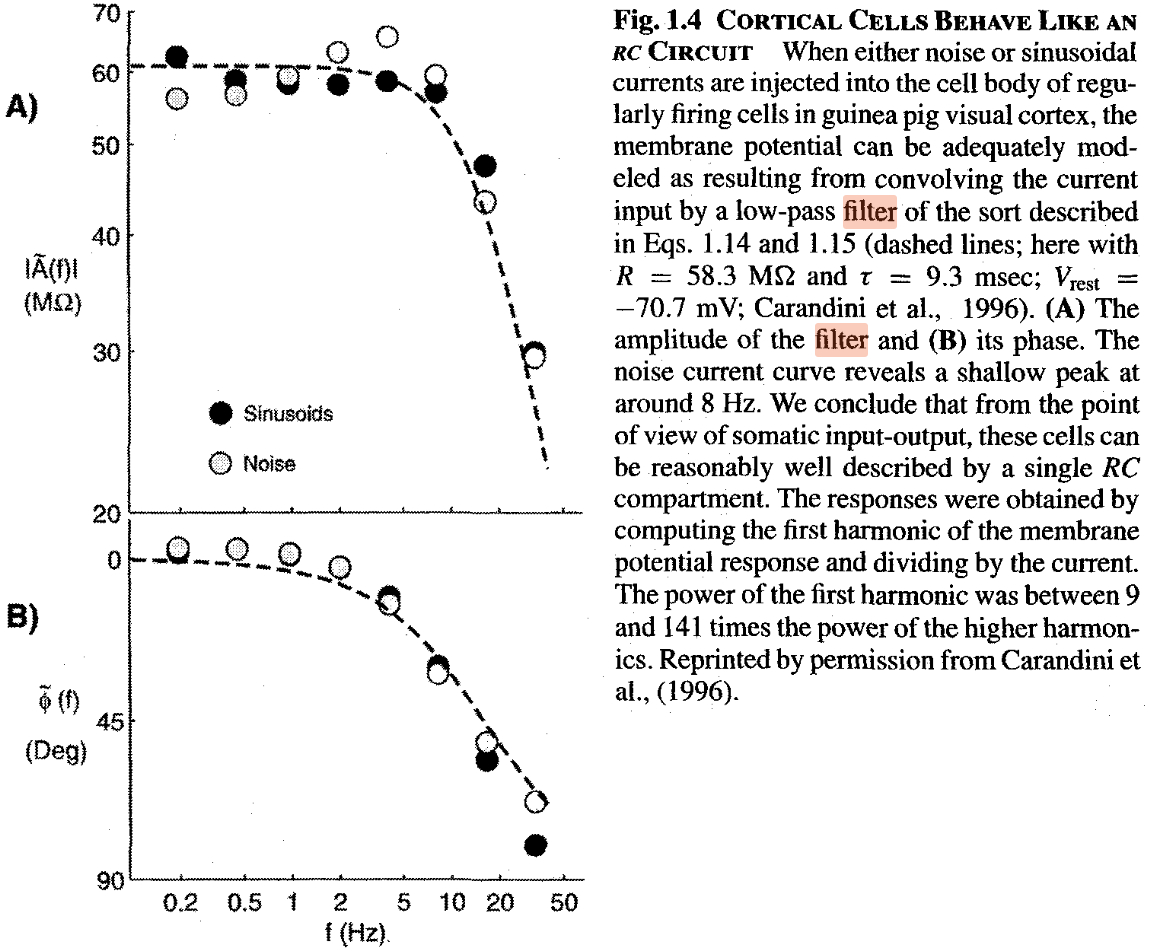
\includegraphics[width=.85\textwidth]{fig/LowPassFilter_Koch.jpg}

\caption{Illustrating the fallacy that neurons represent a low-pass filter. \cite{KochBiophysics:1999} Fig. 1.4 \label{fig:Fallacies-LowPassFilter} }
\end{figure}


Any foreign input current into the membrane, whether it is noise or a sine signal,
increases the momentary and the average resting potential of the membrane,
that is, decreases the probability that the synaptic trigger
arrives at a moment when the synaptic input is enabled.
For how synaptic inputs are enable in function of artificial currents, see our Figure \ref{fig:ArtificialCurrent_AP}.
The arrival time of the spike from the presynaptic neuron is independent
from the operation of the postsynaptic neuron, so the signals arrive at a 'random time'
in the neuron's local time system.
With increasing the frequency of that foreign signal,
more input charge increases the membrane's voltage.
The longer the membrane voltage is above its threshold potential,
the less is the chance to re-open the neuron's synaptic inputs, i.e.,
to receive inputs from the 'regularly firing cell':
the triggers arrive with a high probability in the absolute refractory period.
\index{refractory period}
In the case of varying frequencies, this effect, combined with the finite ion current speed, makes the measured firing rate unpredictable. In a later research, it was noticed that \cite{DepolarizationBianchi:2012}
the too high current blocks spiking (more precisely,
receiving the triggering signal).
\index{spike!blocking}
\index{blocking spikes}

From our conceptual model of generating \gls{AP}
(see Fig. \ref{fig:AP_Conceptual}),
it is immediately clear that although in the 'native mode' of operation,
the falling edge of the \gls{AP}
would result in the membrane's voltage falling below the threshold,
in this way re-enabling synaptic inputs.
However, in 'artificial' mode, the foreign current can keep the voltage above the threshold
(for shorter or longer periods, additionally),
so the synaptic signal cannot enter the membrane, given that
in periods when the membrane has potential value above the threshold,
the synaptic inputs are not enabled; see also Figure~\ref{fig:ArtificialCurrent_AP}.
The synaptic inputs are re-enabled only  later when the membrane's potential is
under the threshold potential when a new synaptic trigger arrives.
That is, the triggering effect
of the "regularly firing cells" is suppressed by the artificially
increased neuronal membrane voltage.
\textit{The effect has nothing to do with the effect 'Low-Pass Filter'}. See also section~\ref{sec:Physics-MembraneElectricity}.


\subsection{Blocking channels by drugs \label{sec:BlockingChannels}}

The commonly accepted belief is that
there are two static bulk concentrations
on the two sides of the membrane and by an unknown mechanism, under the exertion of 'whatnot' forces, without using metabolic energy, ions pass through the ion channels and produce an \gls{AP}.
It is a fact that drugs can drastically affect neuron's  operation. However, there are no observations, that the electrical operation gets blocked, while the thermodynamic one not; that is, that before blocking, electrical and mechanical pulses can be detected, and after blocking, the electrical pulses quit but the mechanical ones persist. Physiology does not want to provide evidence against the 'electrical-only' theory it pre-decided to be correct. \textit{The various mutations of the classical model do not want to know about the experimental evidence that thermodynamic changes (including mechanical waves and thermal changes) accompany the observed electrical operation, while our model states that they are inseparable.} 

If protein-operated ion channels deliver the ions
that cause the \gls{AP}, it must be assumed that the
drug makes the channel (presumably the proteins, which are not required for the channel operation~\cite{HeimburgPhysikOfNerves:2009}) inoperable,
this way blocking issuing \gls{AP}s. 
In fact, when a drug is forcefully injected into a cell, correspondingly to the static view of physiology,
the purpose is to replace
the electrolyte in the bulk with another solution containing the drug. 
In fact, as our dynamic view explains,
the original electrolyte is changed to another one,
and the ion compositions and concentrations change,
thereby due to the vanished gradients, the accelerating voltage across the membrane disappears.
The strong flow (compared to the weak flow
in the resting state) removes
the surrounding ion layers from the surface,
where the electric processes take place; this way dismissing the permanent flows (misidentified as 'specific ion channels').
So, we challenge that the blocking is the effect of the drug
directly on the channels as the old model claims,
and we posit, as follows from our model, that it is the consequence of removing the ions from the electrolyte
and thereby removing the gradients that move the ions across
the membrane.
According to the classic model, the blocked potassium current is expected to flow through the membrane's ion channels.
In other words, the drug blocks the ion channels in the wall
and that invasion stops the current through the \gls{AIS}.
Furthermore, as detailed in section~\ref{sec:Physics-IonSelectivity}, the ion channels' 
selectivity works "primarily" for specific ions,
the rest of ions should continue flowing in, and due to the 
blocked potassium  charge, their intensity should increase.
There is, however, similarly, no such evidence.
%Depending on the conditions, restoring the cell state may require minutes.


\section{Thresholds of initiating AP\label{sec:Physiology-FallaciesAPThresholds}}

As discussed above, ion channels have a voltage threshold that opens
them. We can successfully interpret how the microscopic threshold
of the ion channels forms the macroscopic phenomenon that a voltage
threshold exists for the membrane. Section~17.3 in~\cite{KochBiophysics:1999},
introduces further (current and charge) thresholds. After introducing
the ``slow current'' notion, we can understand that the same voltage
threshold manifests in apparently different thresholds.

As discussed, introducing a sustained current $I_{clamp}$
implies the introduction of a sustained slow current on the membrane's
surface. The sustained current means a sustained presence of ions on the surface, resulting in a continuous increase of potential offset over the resting potential value. As observed, ``the somatic membrane
potential responds with a slight overshoot''. Given that the charge
collection for initiating an 
%\gls{AP}
AP starts at a voltage above the
resting potential, the voltage threshold is reached earlier. The introduced
external current $I_{A}$ is added to the sustained \hyperlink{voltage-clamping}{clamping current}.
The charge delivered by the newly added slow current appears delayed
(after the onset). Depending on the point of the membrane the current
is added, the delay may be up to 1 msec. (As \cite{ActionPotentialGenerationNatrium:2008}
demonstrated, the propagation speed inside a neuron is in the order
of less than 1 cm/s; furthermore, as we discussed, the need to use
electrolyte electrodes can prolong the measured delay time considerably.)
\emph{The current threshold is another manifestation of the voltage
	threshold.}

As we discussed in section~\ref{sec:Physics-SlowCurrent},
the virtue of a capacitive current is used only to imitate the effect
of a slow current: biology has no discrete capacitance. The capacitive
current exists only as a virtual notion in the electric circuit comprising
discrete elements that are considered parallel with the biology-imitating
circuit comprising distributed elements. In the lack of notion of
a ``slow'' current, for ``rapid events'', one may attempt to replace
the ``delayed rectifying current'' with an instantaneous current.
As formulated in section~17.3.5 in~\cite{KochBiophysics:1999}:
``Because we are considering rapid events, the steady-state I-V in
Eq.~17.4 must be replaced by the instantaneous I-V curve''. However,
the rapid events are not rapid enough to make such a replacement in
a differential equation. This replacement results in their Eq.~(17.7)
non-matching values are used. As we explained, Eq.~(\ref{eq:Kirchoff_biological})
formulates Kirchoff's Law in biology. Using \emph{a virtual parameter
	``capacity $C$'' for biological neurons misleads research: introduces
	a nonexisting ``charge threshold'', which exists only due to mismatching
	notions of finite-speed biological circuits with notions of the infinite-speed
	abstract electric circuits}, used to imitate a finite-speed current
in terms of a virtual infinite-speed current.%

\subsubsection{Oscillator type\label{sec:Physiology-HHOscillator}}

If we apply a continuous square wave voltage waveform to an integrator-type electric RC circuit,
we receive an output wave form shown in Fig.~\ref{fig:RCLongWaveform}.
After switching a voltage to the circuit, a charge-up process starts, then the output voltage saturates.
After switching the voltage off, the condenser discharges.
\textit{The time constant $\tau$ for the charge and discharge processes are identical.}
If the time period of the input square wave waveform is made longer
(in the figure with a half-period “$8*\tau$”), the capacitor would then stay fully charged longer
and also stay fully discharged longer.
\begin{figure*}
\centering
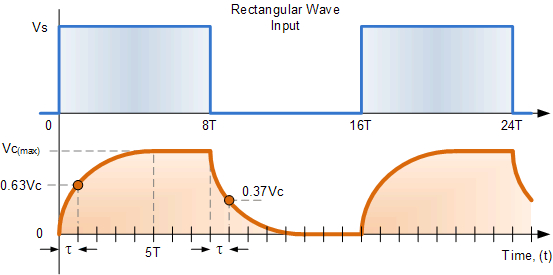
\includegraphics[width=.65\textwidth]{fig/RCLongWaveform.jpg}
		\caption{The output waveform of an integrator-type electric $RC$ circuit
                at a long ($8*\tau$) pulse width square wave input (see Eq.(https://www.electronics-tutorials.ws/) }
		\label{fig:RCLongWaveform}
\end{figure*}

HH measured~\cite{HodgkinHuxley:1952} the time course of the neuronal membrane (i.e., a neuronal $RC$ circuit)
when switched \hyperlink{voltage-clamping}{clamping axonal voltage} on and off.
Their measurement result is shown in Fig.~\ref{fig:ClampingOnOff_HH}.
They experienced a formal similarity with switching a voltage of an integrator-type $RC$ circuit on and off,
compare to Fig.~\ref{fig:RCLongWaveform}, so \textit{they concluded that
the response of the neuronal circuit is identical 
to that of the integrator-type electric $RC$ circuit} (see our discussion in sections~\ref{Physics-OscillatorIntegrator}
and~\ref{sec:PHYSICS_MEASURINGOSCILLATOR}).
They (mistakenly) concluded that the electric equivalent circuit
of a neuron is a parallelly switched electric $RC$ oscillator.
One more evidence that "the success of the equations is no evidence in
favour of the mechanism that we tentatively had in
mind when formulating them". 


\begin{figure}
\centering
\iflatexml
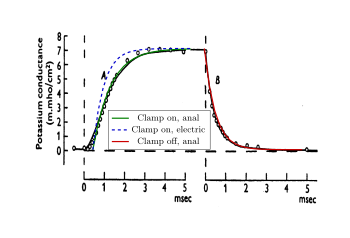
\includegraphics[width=.65\textwidth]{fig/HodgkinHuxleyFig2Simple.svg}
\else
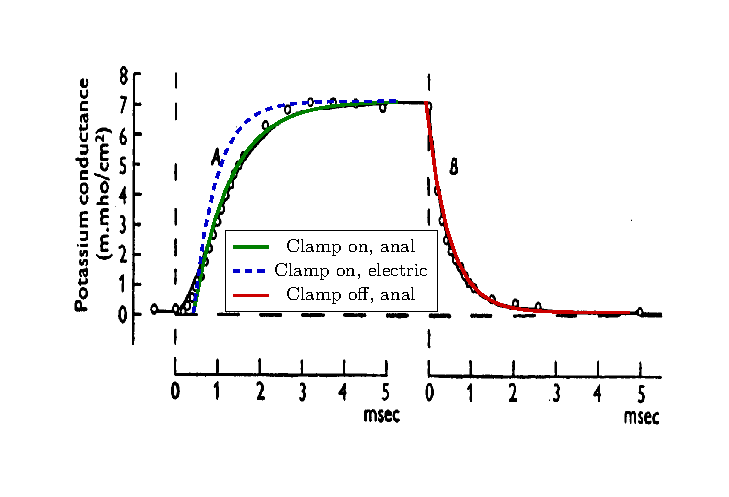
\includegraphics[width=.65\textwidth]{fig/HodgkinHuxleyFig2Simple.pdf}
\fi
\caption{The green and red diagram lines are calculated for the clamping-on and clamping-off case.
he dashed blue line models the case that the neuron is a purely electric system, as opposed to the case of clamping the axonal tube
with ion channels in its wall.  The black bulbs are for measured points.
Moreover, the fitted polynomial line is reproduced from~\cite{HodgkinHuxley:1952}.
}	\label{fig:ClampingOnOff_HH}
\end{figure}

Figure~\ref{fig:ClampingOnOff_HH} shows \textit{two} switch-on diagram lines, with two different $\tau$~time constants. 
The blue line ("electric") is drawn with the measured time constant of the swith-off discharge. 
Acconding to the theory of electricity, the time constants of the falling and rising edge must be the same
in the case of an electric integrator.
The green diagram line (the one fitted to the measured data) correspond to a  different $\tau$~time constant.
The effect was observed by ~\cite{HodgkinHuxley:1952},
but they did not explain and also did not interpret it. 
Although their fitted polynomial nearly hides the effect, a little "hump" at around $3\ ms$ can be observed.
The reason is that the charge-up current is not constant, it also has a time course; despite that they stabilized the voltage. 

  The different time constants should have been a warning sign for HH that
  \textit{the measured effect differs from the one they had in mind}.
%
They wanted to believe and demonstrate that they have measured the output signal
of a serial $RC$ circuit.
With the evaluation of their measurement, they suggested some wrong hypotheses 
\begin{itemize}
\item They misidentified the current as \textit{the 
change of conductance}. No conductance change happens, only a condenser 
changes and discharges. They worked with a condenser, not with a resistor.
\item They meticulously observed and measured that the time contants $\tau$
of the exponential charge-up and discharge processes are different;
but did not care that they should be indentical and also did not care of the "hump".
\item They measured the resulting charge-up composite process. As we explain in section~\ref{sec:Physics-Current},
before switching the clamping voltage, there is no charge carrier 
inside the axonal tube; first, the ions must diffuse into the axon.
\item They fitted the rising time course with a polynomial, hiding 
that it comprises a saturating voltage of the condenser, that 
the current through the axon also saturated with a different time constant, 
and at the begining the line had a zero current contribution.
\end{itemize} 
 

On the one side, they underpinned that our equations \ref{eq:I_Source} and \ref{eq:I_Drain}
describe correctly the axonal chargeup current and discharge currents, respectively.
On the other, as they noticed that the time constants of the two processes are significantly different
(see the green and the dashed blue diagram lines), underpinned that
the axonal charge production mechanism significantly changes
the axonal source current. The green line has significantly slower rise
since the axonal current only gradually increases after switching the clamping on.
Without that current change, the charge-up current would follow the blue line.
Unfortunately, there are three physical processes, with similar time constants.
One, that they wanted to demonstrate is the steady state:
the current leads to a saturated current. 
Two, that the \hyperlink{voltage-clamping}{clamping "creates" charge carriers} in the axon,
so the charging current changes.
Three, the initial switch-on creates a voltage gradient on the membrane,
so an action potential is also started.
\index{voltage gradient}
 

Their equations more or less precisely describe
the features of the wrong oscillator type and those of the
non-existing $K^+$ current introduced for compensating for the wrong oscillator selection.



\section{The cable equation\label{sec:Physics-CableEquation}}

Even though axons are tubes and deliver
charge, \emph{we must not describe that process using the telegrapher's
	equation because of fundamental differences}. The electrical telegraph
cable continuously loses charge (current is leaking due to the specific
resistance of the cable).  In a biological cable, no potential
is switched to the end of the cable, and no leaking current is present, furthermore, the nature of resistance differs from
that of solids. The relevant physical
entities are the potential and concentration gradients, as described by
the Nernst-Planck equation, instead of the electrical and magnetic gradients,
as described by the Maxwell equations.
The charge moves autonomously (more precisely, it is described by the damped oscillation of the electrolyte), and has nothing to do with a coordinated action of ion channels. It is just an unfortunate accidence that the speed of solitons and the conduction velocity fall in the same order of magnitude.

%\subsubsection{Cable equation\label{Physiology-HHCableEquation}}

Selecting the wrong oscillator type (actually, assuming distributed parallel
oscillator circuit) and the wrong electrotonic model
leads to somewhat surprising consequences,
such as using the telegrapher equations in a wrong way for
describing neuronal transfer.
By using the cable equation, as Hodgkin and Huxley attempted~\cite{HodgkinHuxley:1952}, led to
\index{cable equation}
numerical difficulties, and they faced the principal problem: their
equations assumed infinitely fast electric interaction, and they attempted
to combine them with the (unknown) finite macroscopic speed of current
in neuronal telegraph cables. The validity of using cable equations
for biological objects is at least doubtful: deriving a telegrapher
equation assumes applying an external potential to the cable filled
\index{telegrapher's equations}
with charge carriers, and in the case of biological membranes neither
external potential nor permanently present charge carriers exist.
Furthermore, the cable equation assumes continuous current outflow
(a distributed resistance), which is not true for the neuronal membrane
(current flows only toward the \gls{AIS}).
\index{cable equation}
\index{telegrapher's equations}


